%%---
%\begin{figure*}[ht!]
%	\centering
%	\hspace*{\fill}
%	\subfloat[]{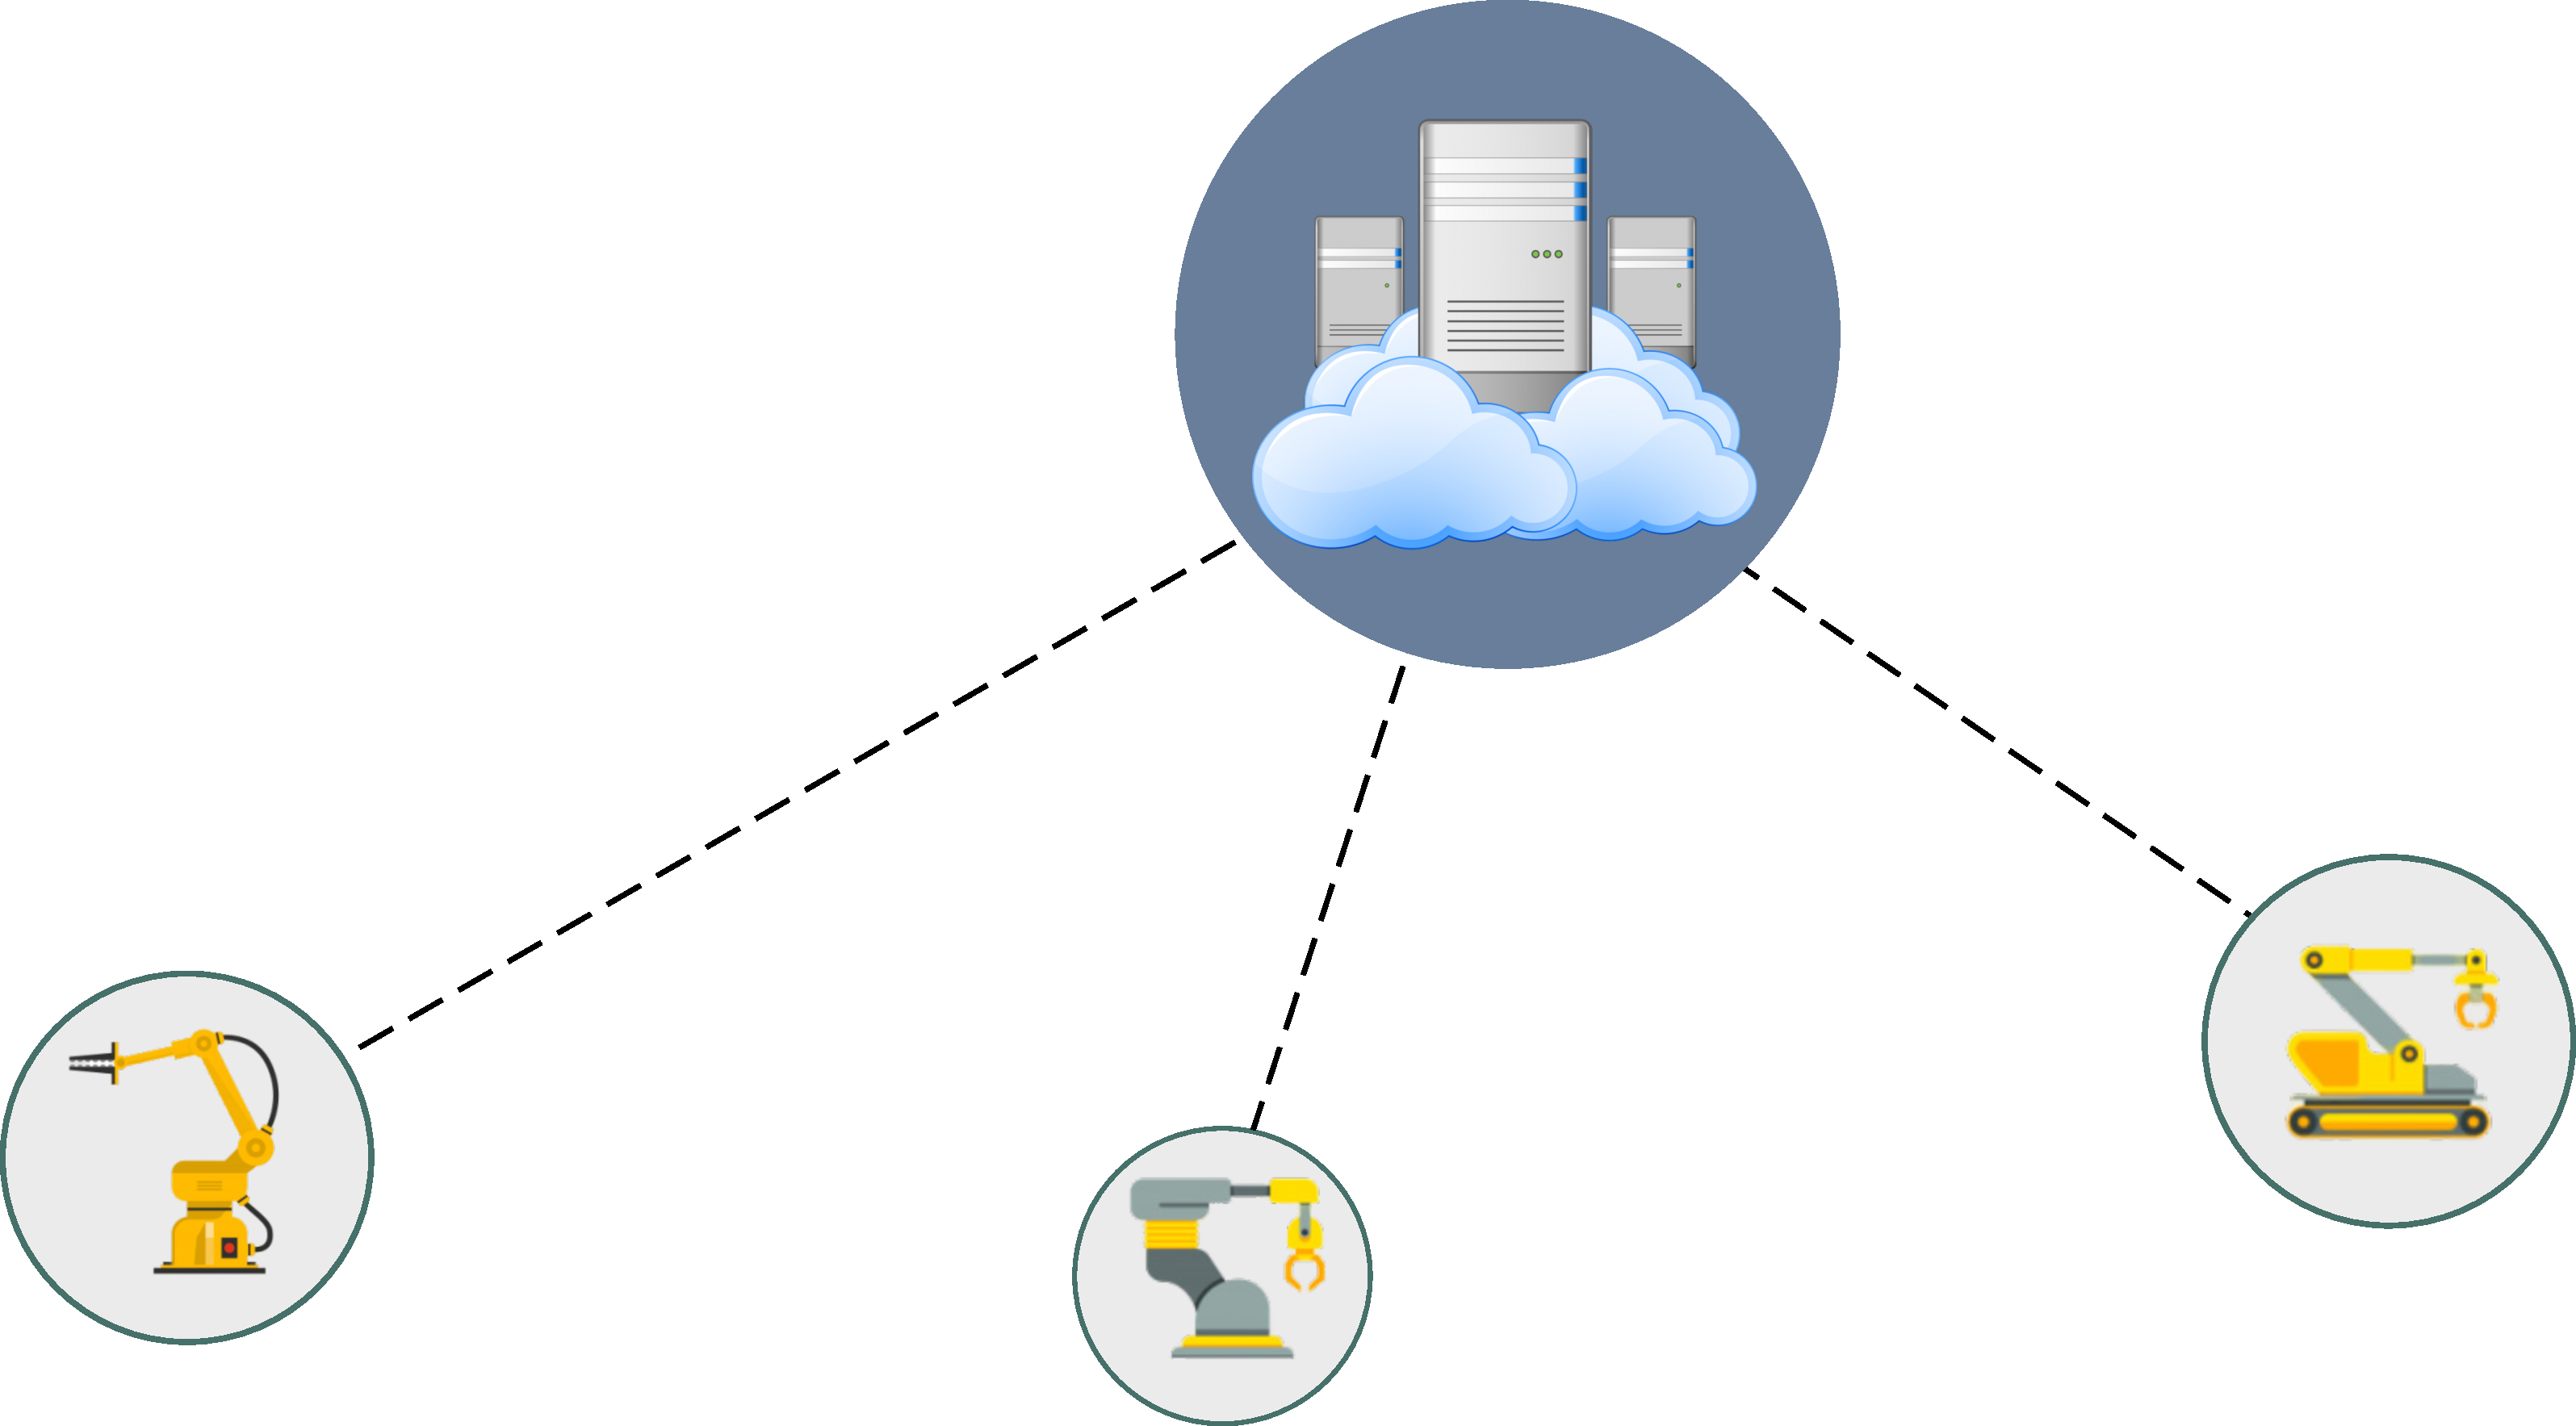
\includegraphics[width= 0.90\columnwidth]{fig/isolated_learning.pdf} \label{fig:isolated_learning}}
%	%\hspace*{\fill}
%	\hfill
%	\subfloat[]{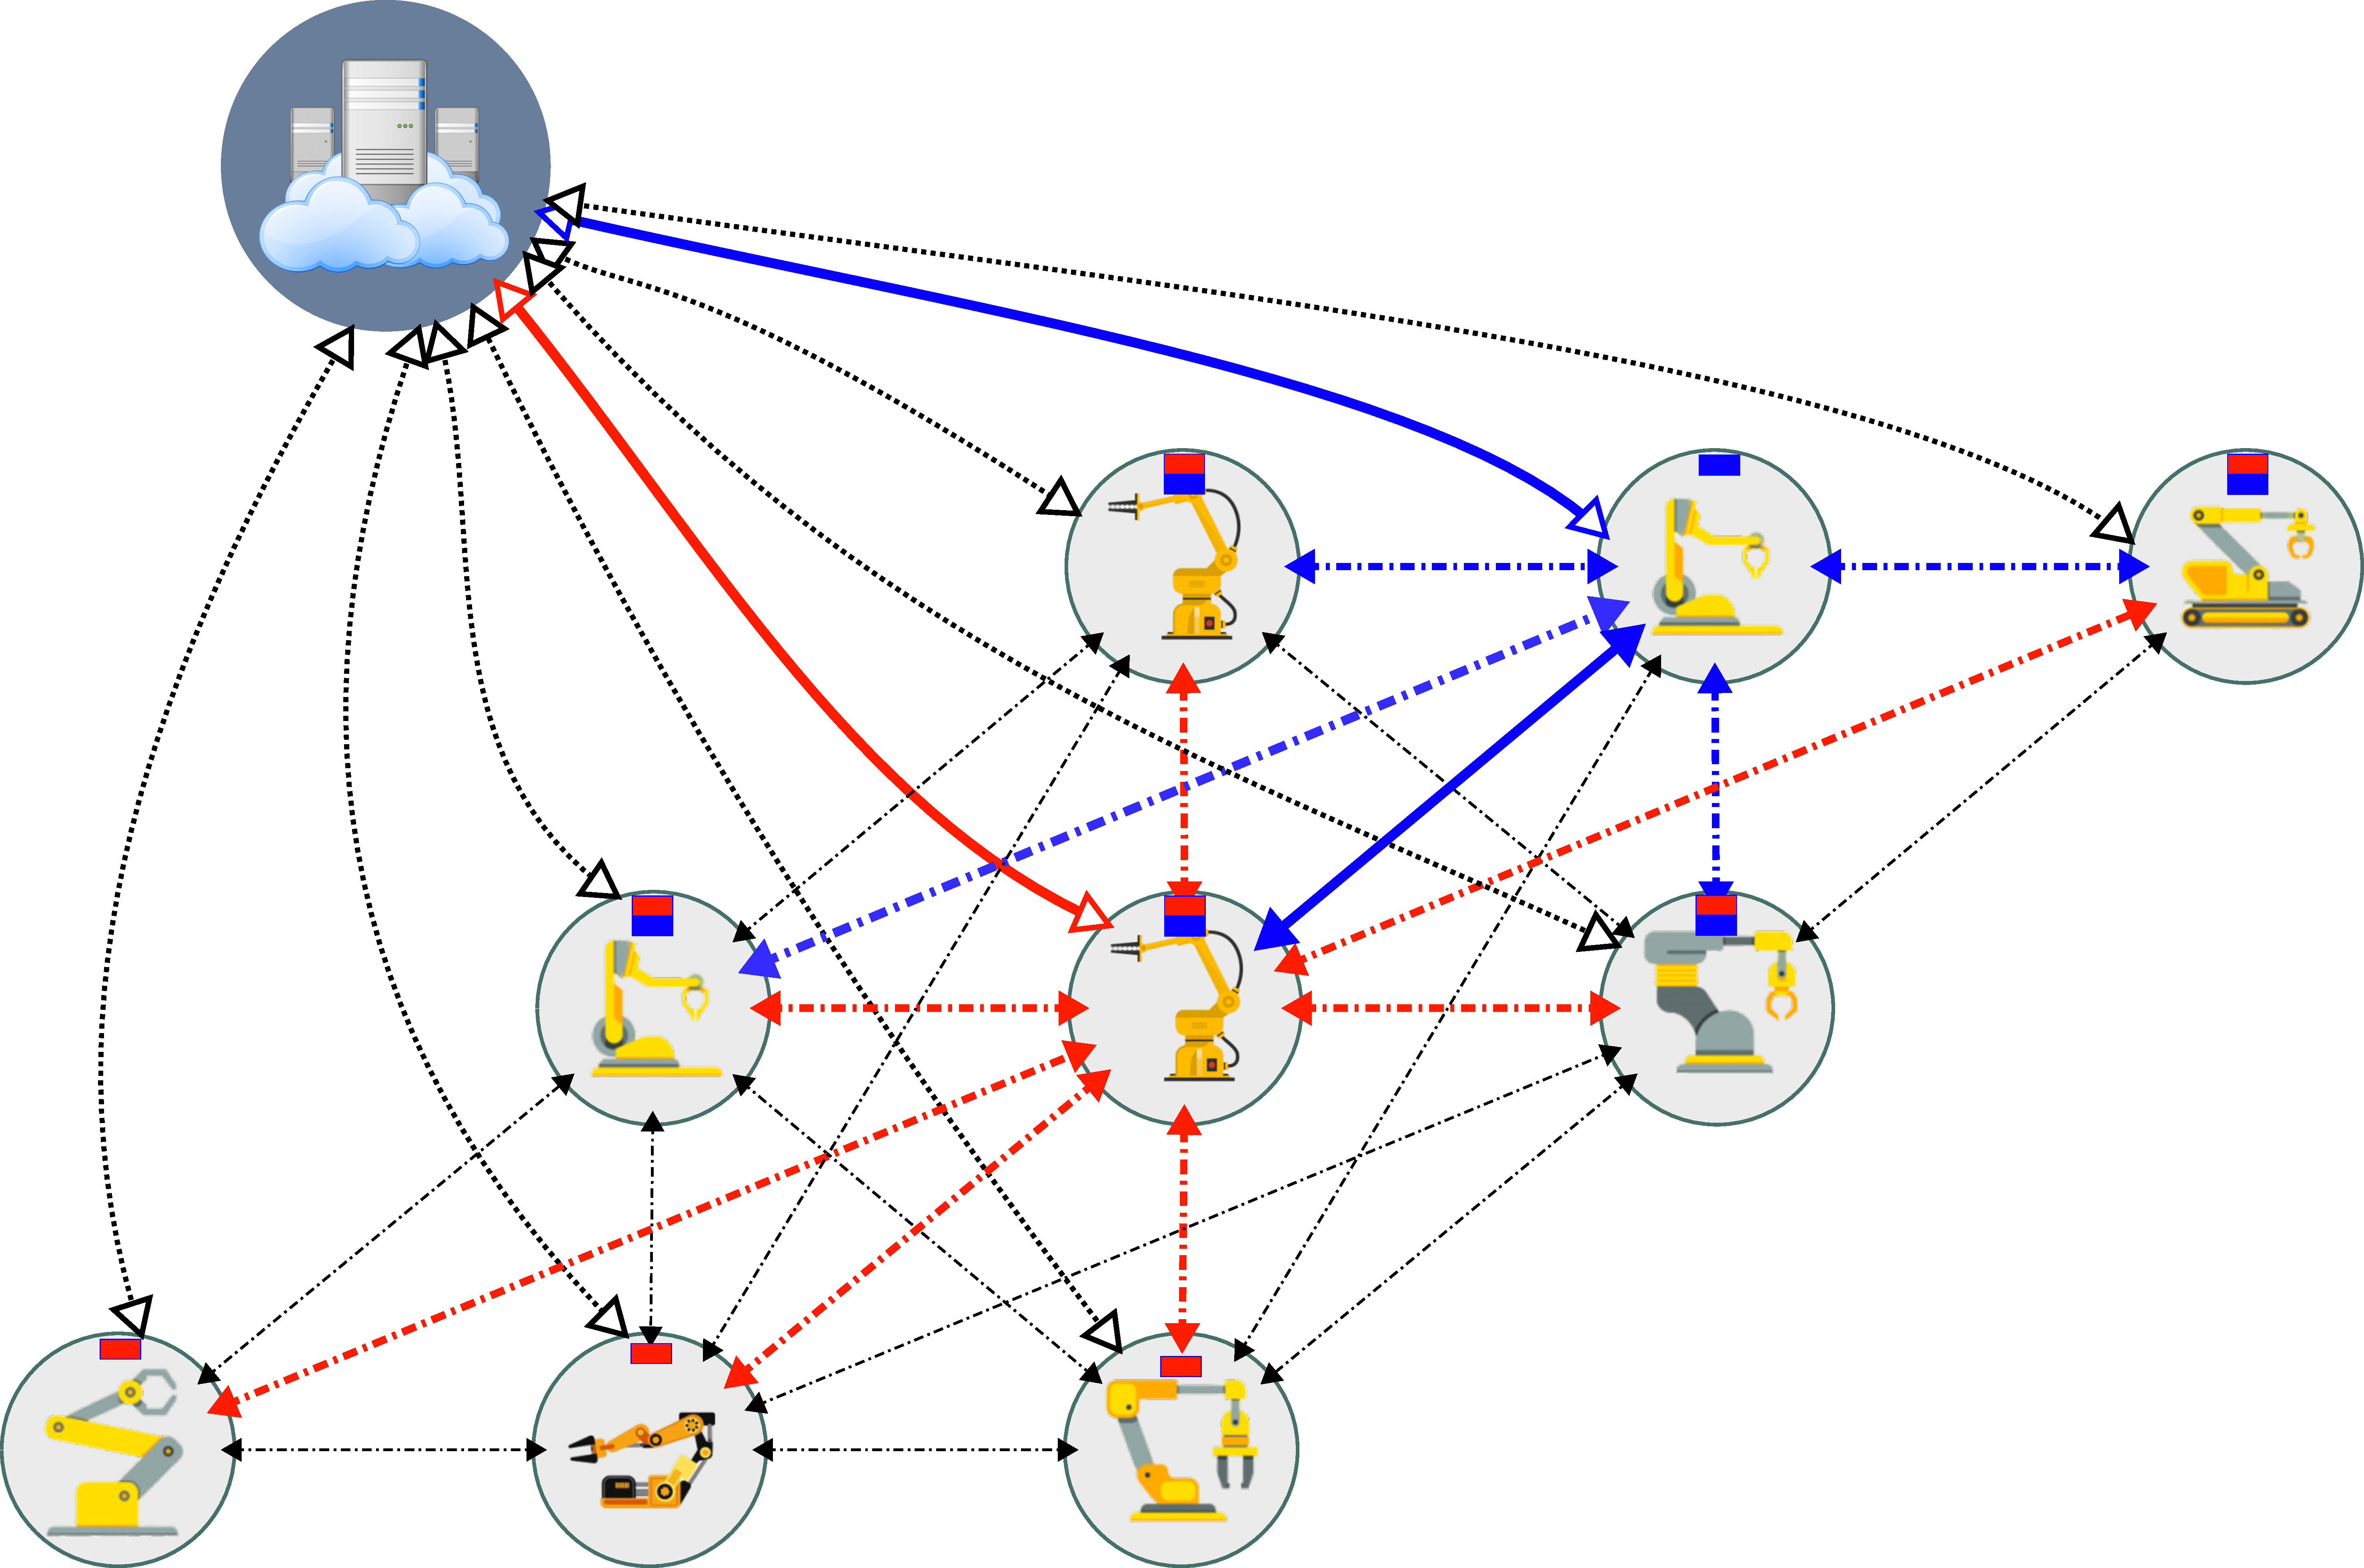
\includegraphics[width= 0.80\columnwidth]{fig/collective_learning_v3.pdf} \label{fig:collective_learning}}
%	\hspace*{\fill}
%	\caption[] {\label{fig:learning_paradigms} Learning paradignms: \subref{fig:isolated_learning} isolated learning and \subref{fig:collective_learning} collective learning. }
%\end{figure*}
%%---

%The ability to share information so efficiently that the ideas of individuals can be stored within the collective memory of communities and can accumulate through generations. 
%
%The process through which different actors develop a collective mind which concerns how they use their own network and interactions as culture-based contextual conditions for everyday learning processes including opportunities to use their concrete experiences, knowledge, and skills. It involves horizontally based cooperation between different actors in a local or organizational setting or the mobilization of resources in a broader context as such to initiate a learning-based process of innovation and change
%
%Collective learning is a complex concept that is variously defined. It is generally conceptualized as a dynamic and cumulative process that results in the production of knowledge. Such knowledge is institutionalized in the form of structures, rules, routines,norms, discourse, and strategies that guide future action. Learning emerges because of interactive mechanisms where individual knowledge is shared, disseminated,  diffused,  and  further  developed  through relational and belonging synergies. 
%
%Collective learning, therefore, represents a macro concept that addresses learning at the levels of the team,the organization, and society. 
%
%An important distinction is made between individual learning and collective learning. Individual learning tends to be conceptualized as an information system where learning is interpreted, retained, and retrieved by individuals. Collective learning is viewed as a more macro-level concept that emphasizes the synergy and advantages of the collective element
%
%Central to collective learning is the notion that the collective is enhanced in three ways: (a) it achieves the capacity to restructure and to meet changing conditions; (b) it can add and use skills, knowledge, and behaviors; and (c) it becomes highly sophisticated in its capability to deal with feedback and reflect on its actions.
%
%Different types of collective learning are highlighted in the literature:
%\begin{itemize}
%	\item Aggregate learning is conceptualized as the aggregation of learning gained though trial and error at the individual level. The emphasis is on individual learning processes rather than any collective perspective. Aggregate learning may give rise to fragmentation and individualization rather than inclusion and collectivity
%	\item Group learning focuses on the processes that a group uses to acquire new skills, knowledge, ways of interacting, change patterns between group members, standard operating procedures, and behavioral routines
%\end{itemize}
%
%Camagni (1991) suggests that collective learning is not simply the acquisition of information, and that the availability of information is not a central issue.Instead, it is the process by which available information becomes usable knowledge that is the main focus.

% ===================================================================================================
%                                                 |                                                 |
%                                                 |                                                 |
% -------------------------------------------- SECTION ---------------------------------------------|
%                                                 |                                                 |
%                                                 |                                                 |
% ===================================================================================================
\section{A learning paradigm for embodied AI}
%---
\begin{figure*}[!t]
	\centering
	\hspace*{\fill}
	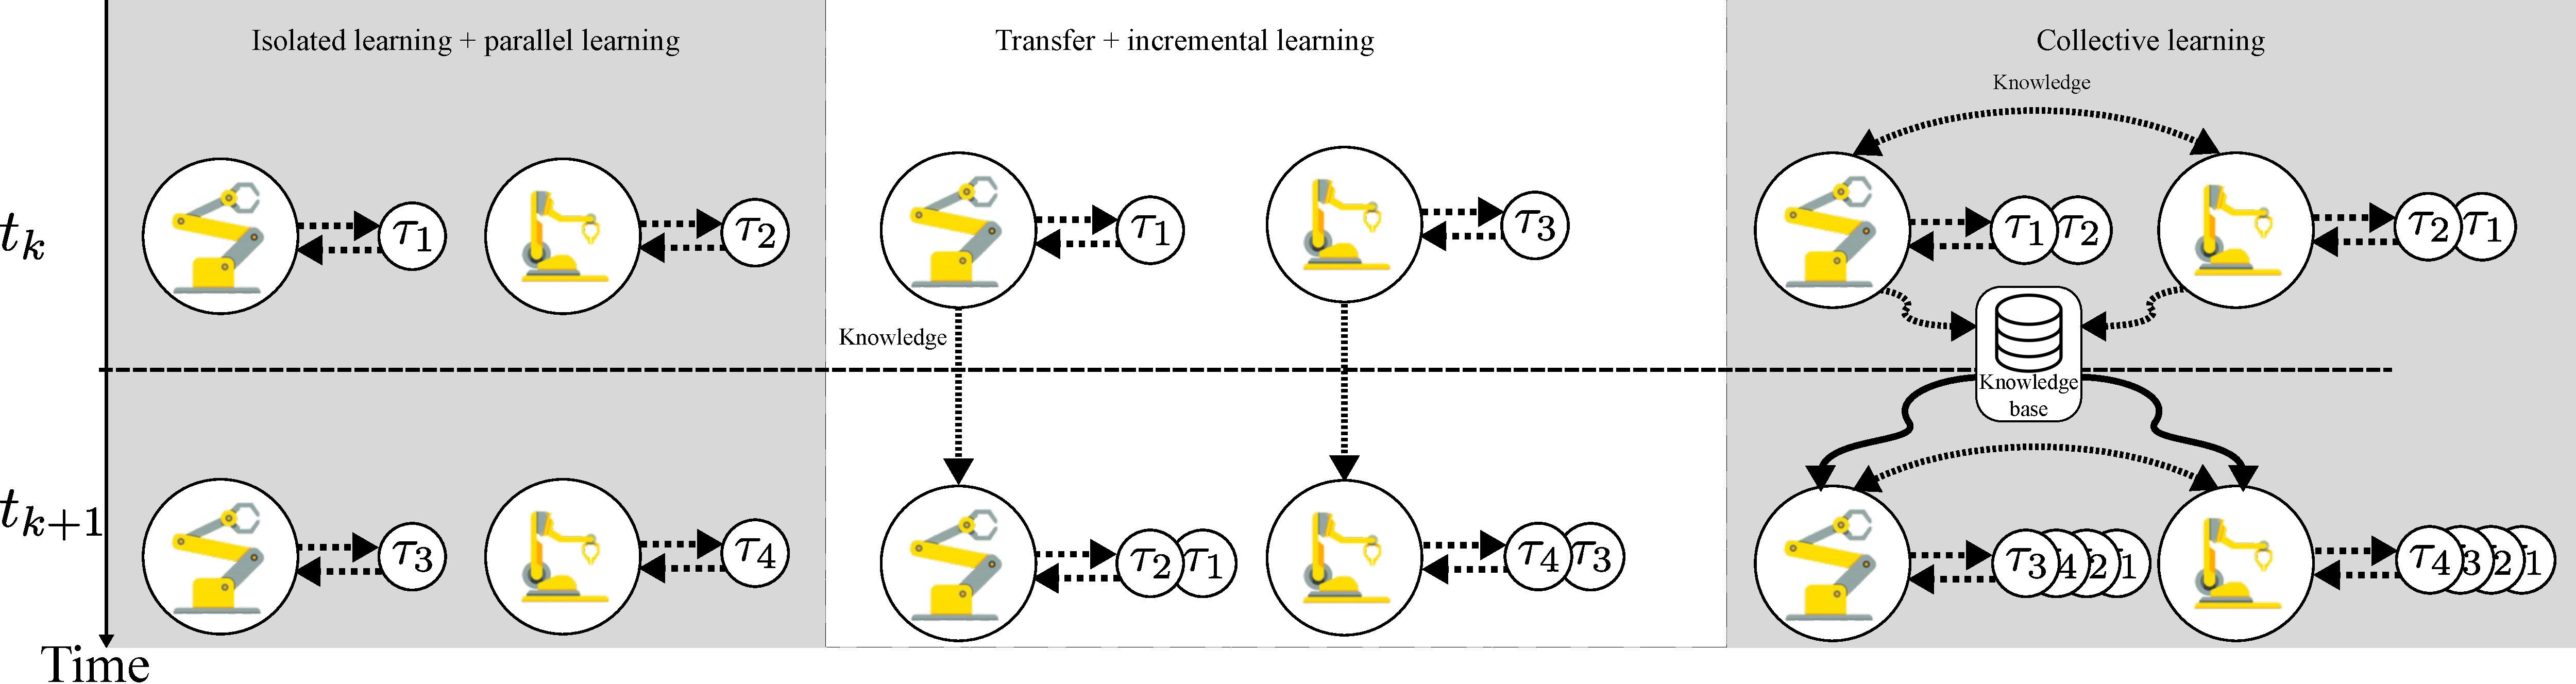
\includegraphics[width= 0.95\textwidth]{fig/learning_paradigms_v3.pdf} \label{fig:isolated_learning}
	\hspace*{\fill}
	\caption[] {\label{fig:learning_paradigms} Learning paradigms.}
\end{figure*}
% ---
% SUBSECTION ========================================================================================
\subsection{Learning paradigms}
Among all the learning schemes, four paradigms are distinguishable: isolated, transfer, incremental, and collective. 

In \textit{Isolated Learning}, the agent tries to learn a given task as a single problem, i.e., it acts alone and measures its performance by observing how successful it was in accomplishing the task. This process repeats until a convergence criterion is reached. The model trained by the agent is specific for each task and, therefore, is trained from scratch for every new task. $N$ agents training in parallel will learn $N_1$ different tasks at the same time, one model each. In the end, each agent will only be able to optimally execute one task. If training is repeated for a new task there is no knowledge aggregation, one agent will still only be able to accomplish only one task.
%\textcolor{red}{Here most of the improvement in speed is attributed here to more potent hardware rather than to more efficient learning algorithms}. 
% \textcolor{red}{incremental learning proposes that the model knowledge acquired by one agent in a set of tasks can be used to bootstrap the learning of a new similar one. This implies that if a set of relevant tasks is learned by a model there might be no need for further training.}

\textit{Transfer Learning}, on the other hand, considers as a basic premise, that a given learning system can leverage knowledge to solve a task from previous experiences with similar tasks. This implies that if a set of relevant tasks is learned by a single model there might be very little remaining training effort or even no need for further training at all in order to generalize for other similar tasks. $N$ agents training in parallel will learn a single model for $N_1$ different tasks at the same time. In the end, each agent will be able to sub-optimally execute $N_1+M_1$ tasks, where $M_1$ is the number of tasks that share high similarity with the original $N_1$ tasks trained. \hl{Similar to isolated learning, if training is repeated for a new set of tasks there is no knowledge aggregation, one agent trained in $N_2$ tasks will still be able to sub-optimally execute $N_2+M_2$ task.}     
% It is common to see in the literature that the learner is composed of a single-agent and, therefore, it is only possible to learn from the agent's own previous experience. 

\textcolor{black}{\textit{Incremental Learning}, proposes that the learning process should be able to learn as tasks comes in, i.e., the set of tasks that the model can solve should expand by incrementally updating the model to perform better in the new task without losing much performance in the already learned ones. $N$ agents training in parallel will learn $N_1$ different tasks at the same time, one model each. In the end, each agent will only be able to optimally execute one task. However, if training is repeated for a new set of $N_2$ new tasks, knowledge should aggregated. Therefore, each agent would be able to sub-optimally execute 2 tasks. This paradigm can work by itself but it is normally combined with \textit{Transfer Learning} (\textit{Transfer + Incremental Learning}), meaning that there is a shared model that learns all trained tasks at the same time and is able to incrementally learn new tasks.} % A logical way to improve the learning speed is to use a multi-agent setting. To outperform the single-agent case it is expected that some form of parallelization is explored, the most simple approach is to have a centralized learning model and distribute different attempts among all agents, this would, potentially, already accelerate the learning by the number of agents in the system. If, for example, some smart exploration and task segmentation scheme is used, the acceleration can increase by many times more. 

% \begin{figure}[!t]
% 	\centering
% 	\hspace*{\fill}
% 	\subfloat[]{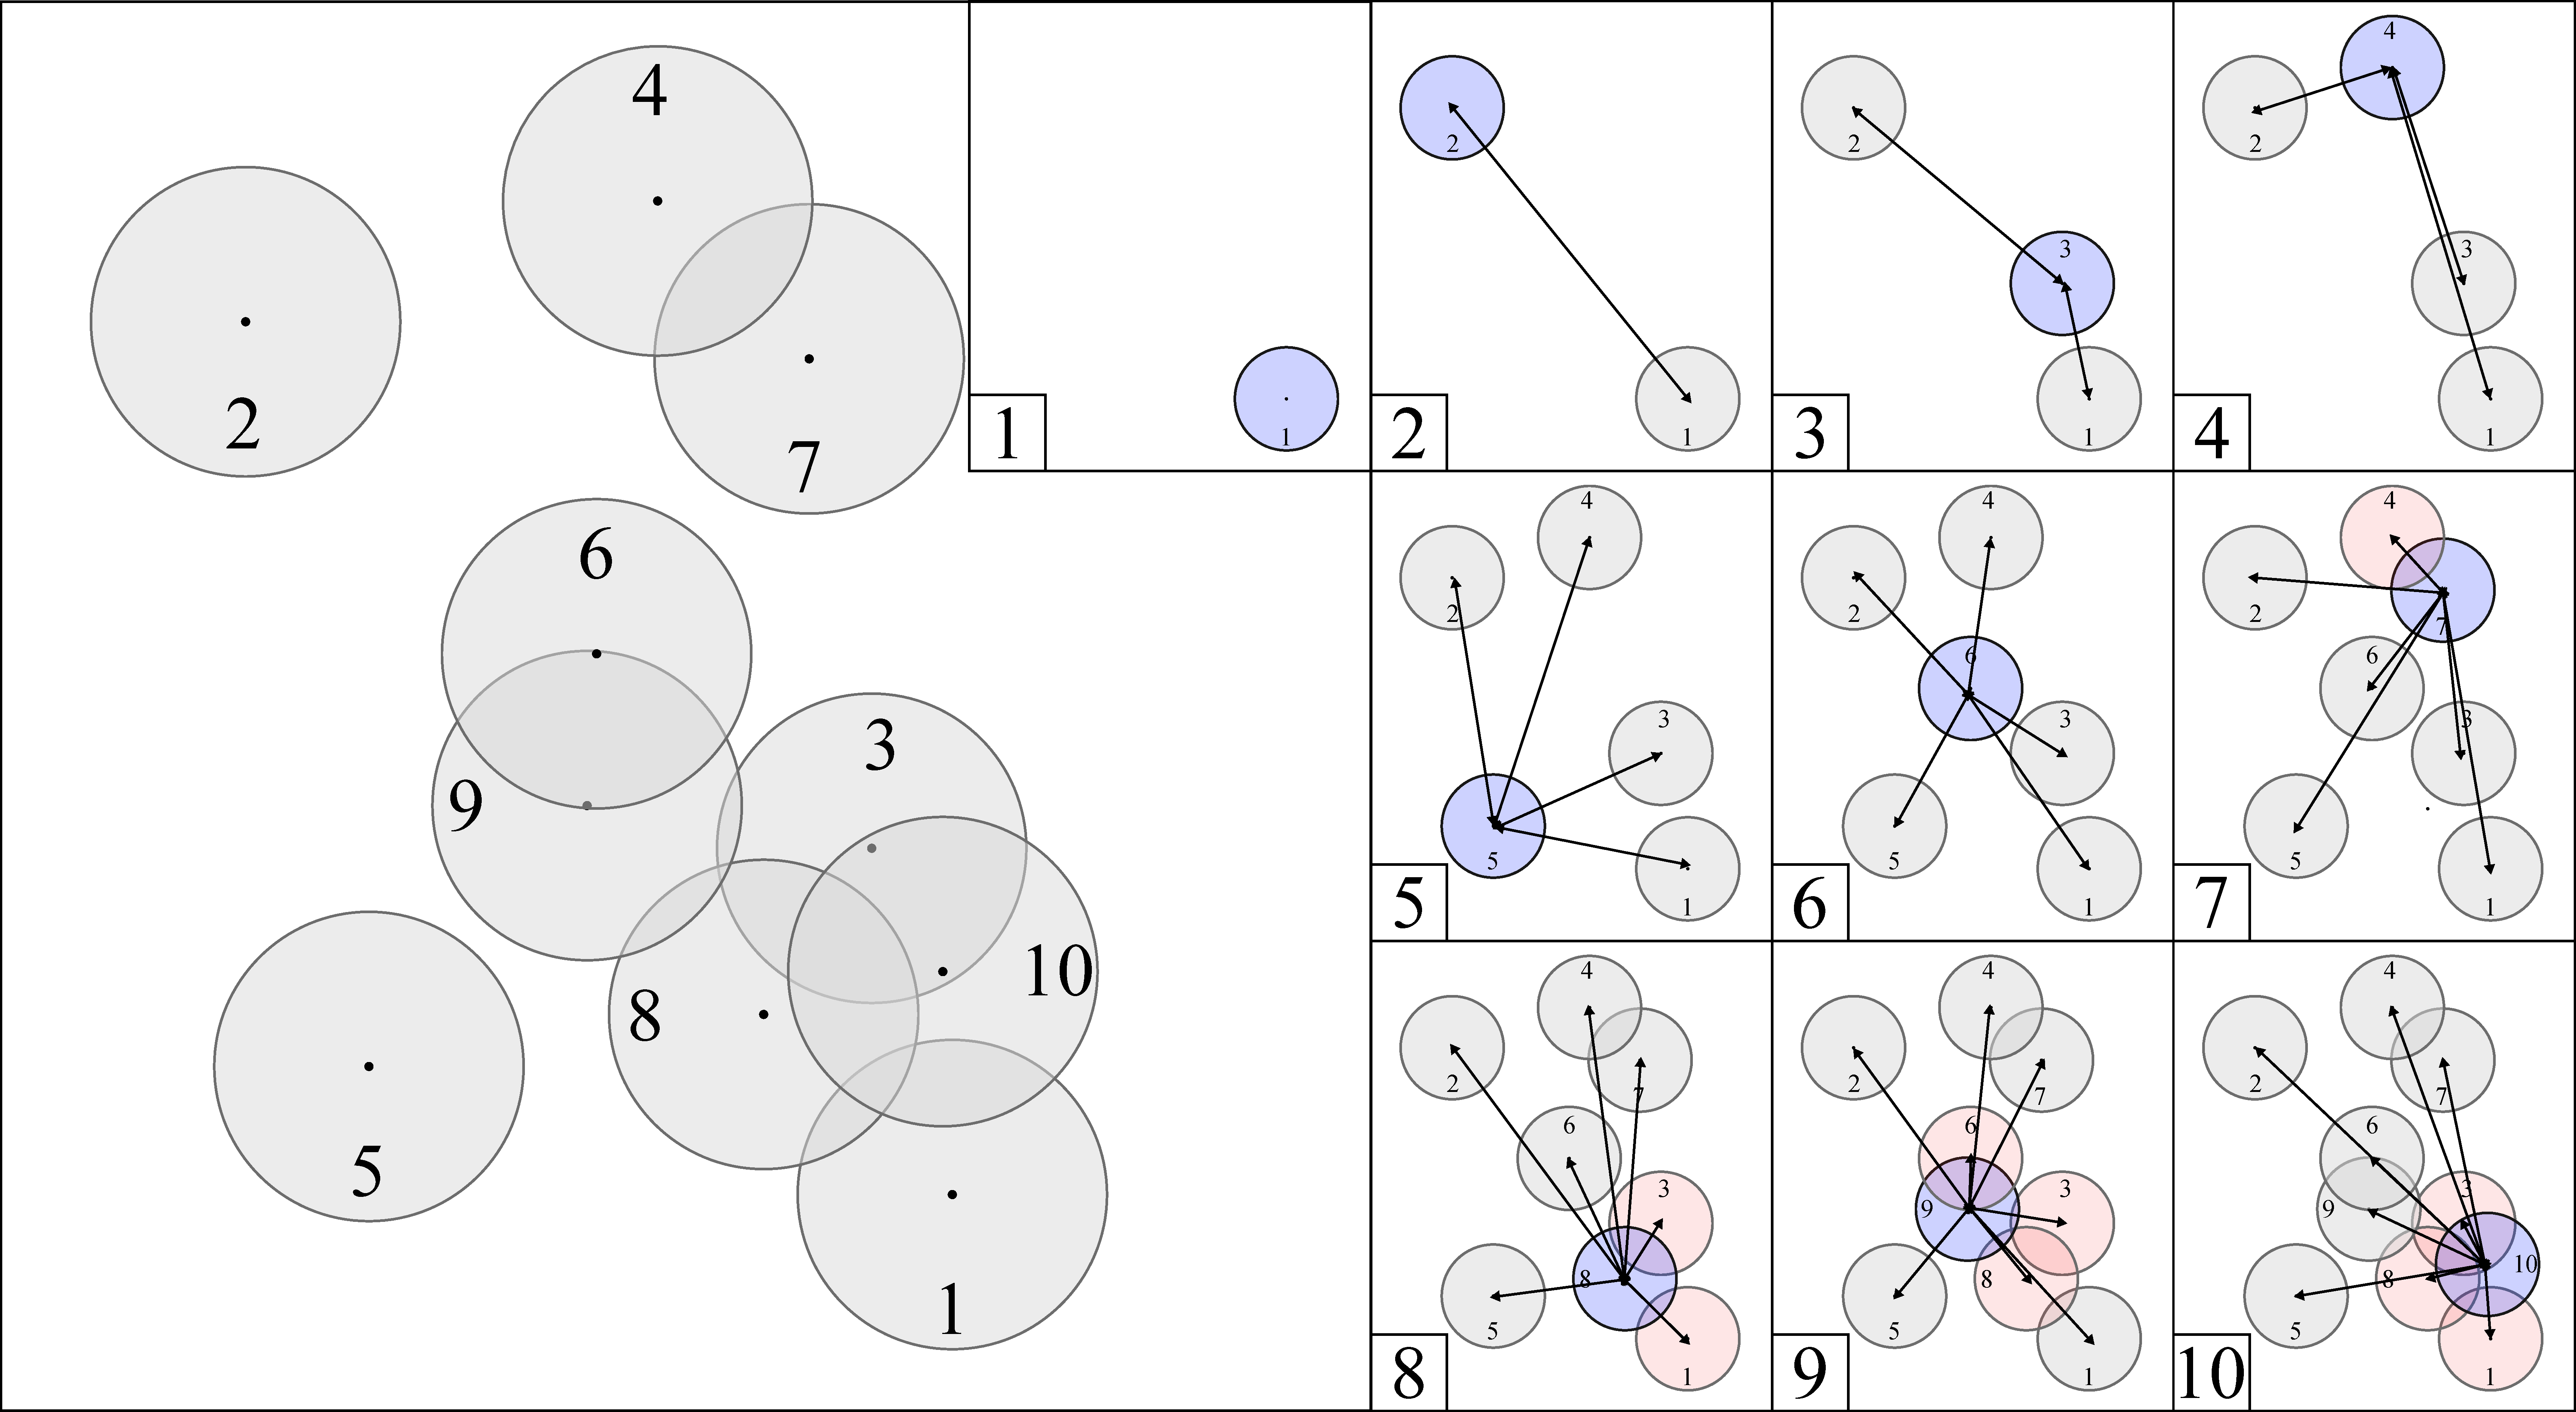
\includegraphics[width= 0.99\columnwidth]{fig/task_areas_v2.pdf} \label{fig:isolated_learning}}
% 	\hspace*{\fill}
% 	\caption[] {\label{fig:trasfer_learning} Transfer learning. The illustration shows a series of tasks learned sequentially. The intersection between a target task and other tasks is shared knowledge; the intersection between tasks in the pool if known tasks in redundant knowledge.}
% \end{figure}



Finally, \textit{Collective Learning} extends \textit{Transfer + Incremental Learning} by assuming that multiple agents will take part in the learning process. It proposes that partial knowledge about the task should be constantly shared among all other agents, even before any task is successfully learned. %Thus, Collective Learning is an umbrella term used to describe the subset of learning algorithms that can leverage on a multi-agent causality inference with a centralized learning model. 
The general high-level goal is that agents who are learning similar tasks in parallel can share common knowledge, during training episodes, despite not yet been able to accomplish their own tasks. This can, potentially, critically speed up the training process. The key idea is that each agent experience can aggregate in the learning process of the others by providing insights on how to perform part of the task, assuming there exists potential transferability among them. Fig.~\ref{fig:learning_paradigms} illustrates the different learning paradigms.

% SUBSECTION ========================================================================================
\subsection{Collective learning for embodied AI}
\textcolor{black}{As we mentioned in Sec.~\ref{sec:intro}, embodied AI systems will be a core element of the smart factory. Moreover, the communication and cloud processing of the smart factory and Industry 4.0 will be at the disposal of these systems. Furthermore, as we saw in Sec.~\ref{sec:robots_challenge}, there will be legions of robots performing several different tasks at any given time. Considering these, it is immediately evident, that relying on isolated learning in this setup is senseless as it would not exploit the infrastructure and would directly contribute to more computational demands (see \textbf{challenge 1}). Similarly, although offering a better perspective, transfer + incremental learning would benefit from the previous experience collected by the agents but would not take full advantage of the potential for partial knowledge learning among agents, provided by the numbers of robots learning and executing related tasks. Therefore, we see in collective learning the natural paradigm to exploit the full potential of the smart factory infrastructure and leverage all the real-time collected knowledge of all the networked embodied AI agents in a synergistic manner.}

To formalize this idea, let $ \left\lbrace \rho_i \right\rbrace_{i=1}^{m} $ be a set of robotic agents that defines a community of robots. In collective learning, the different robotic agents $ \rho_i $ develop and accumulate dynamically a common mind (body of knowledge) via networked interactions where individual experience, knowledge and skills are disseminated to all the other elements in the collective. Information flows vertically as previous knowledge is passed on, as well as horizontally by sharing concurrent experience between agents. Via these mechanisms, knowledge can be replicated, complimented and further developed. We take from \cite{Garavan2012CollectiveLearning} two notions central in collective learning that are applicable to the embodied AI agents:
% ---
\begin{enumerate}
	\item Capability to restructure and meet changing conditions
	\item Aggregation of skills, knowledge, and behaviors
\end{enumerate}
% ---
Collective learning contrasts with the previously discussed incremental learning in that a single agent $ r_i $ can aggregate only so much knowledge via trial and error and is limited by a sequential learning structure. Learning collectively, on the other hand, enforces parallelization of knowledge acquisition via the concurrent learning and sharing of all agents as they acquire new skills, knowledge. Moreover, collective learning involves not only the information acquisition, but also how this information is brought to use to form and develop knowledge. 

Collective learning is not only a promising research direction but, in our opinion, has the potential to be a unifying solution to the grand the challenges posed by embodied AI. By incorporating new mechanical designs as agents in the learning pipeline it is possible to iteratively evaluate the energy efficiency of proposed solutions and select the best ones as reference designs for future manufacturing processes, therefore, promoting a cyclical optimization towards a semi-optimal general design.

In the next section we delve more deeply into the mathematical formulation of the elements we just described. 